\documentclass[11pt,a4paper]{article}

% =========================================================================
% PACKAGES & DOCUMENT HYGIENE
% =========================================================================
\usepackage[utf8]{inputenc}
\usepackage[top=20mm,bottom=20mm,left=22mm,right=22mm]{geometry}
\usepackage{amsmath,amssymb,amsfonts}
\usepackage{booktabs}
\usepackage{tabularx}
\usepackage{graphicx}
\usepackage{xcolor}
\usepackage{hyperref}
\usepackage{fancyhdr}
\usepackage{titlesec}
\usepackage{enumitem}
\usepackage{tcolorbox}
\usepackage{microtype}
\usepackage{caption}

% Semantic Color Palette
\definecolor{brandblue}{HTML}{005691}
\definecolor{brandcyan}{HTML}{0891B2}
\definecolor{darkslate}{HTML}{0F172A}
\definecolor{safegreen}{HTML}{10B981}
\definecolor{warnamber}{HTML}{F59E0B}
\definecolor{breachred}{HTML}{EF4444}
\definecolor{lightgray}{HTML}{F8FAFC}
\definecolor{bordergray}{HTML}{E2E8F0}
\definecolor{codebg}{HTML}{F1F5F9}

% Hyperlink Setup
\hypersetup{
    colorlinks=true,
    linkcolor=brandblue,
    citecolor=brandblue,
    urlcolor=brandblue,
    pdfauthor={Team UFTB-VORQEN},
    pdftitle={ColdChain Technical Documentation - BUBT FastRobox 1.0 Hackathon}
}

% Header and Footer
\pagestyle{fancy}
\fancyhf{}
\fancyhead[L]{\small \textbf{FastRobox 1.0 IoT Hackathon 2026} $|$ IEEE BUBT Student Branch}
\fancyhead[R]{\small Team: \textbf{UFTB-VORQEN}}
\fancyfoot[L]{\small ColdChain: Vaccine \& Medicine Storage Monitor}
\fancyfoot[R]{\small Page \thepage}
\renewcommand{\headrulewidth}{0.5pt}
\renewcommand{\footrulewidth}{0.5pt}

% Section Titles Styling (Single Column)
\titleformat{\section}{\Large\bfseries\color{brandblue}}{\thesection.}{0.6em}{}[\titlerule]
\titleformat{\subsection}{\large\bfseries\color{darkslate}}{\thesubsection.}{0.5em}{}
\titleformat{\subsubsection}{\normalsize\bfseries\color{brandcyan}}{\thesubsubsection.}{0.4em}{}

% Custom Callout Boxes
\tcbset{
    colback=lightgray,
    colframe=brandblue,
    arc=2mm,
    boxrule=1pt,
    left=4mm,
    right=4mm,
    top=3mm,
    bottom=3mm
}

\captionsetup{
    font=small,
    labelfont={bf,color=brandblue},
    justification=centering,
    skip=6pt
}

% =========================================================================
% DOCUMENT CONTENT
% =========================================================================
\begin{document}

% --- TITLE BLOCK (NO HEADER IMAGE, CLEAN PROFESSIONAL TYPOGRAPHY) ---
\begin{center}
    {\LARGE \textbf{\color{brandblue}ColdChain: Autonomous IoT Cold-Chain Monitoring \& Predictive Bio-Thermal Safety Platform}}\\[8pt]
    {\large \textbf{Comprehensive Engineering Documentation \& Technical Implementation Report}}\\[5pt]
    {\normalsize \textbf{Event:} BUBT FastRobox 1.0 IoT Hackathon 2026 \quad$|$\quad \textbf{Organized by:} IEEE BUBT Student Branch}\\[4pt]
    {\normalsize \textbf{Team Identity:} \textbf{\color{brandblue}UFTB-VORQEN} \quad$|$\quad \textbf{Challenge Track:} 100-Point IoT Problem Statement}\\[4pt]
    {\small \textbf{GitHub Repository:} \href{https://github.com/Masud744/FastRobox1.0_Hackathon}{\texttt{github.com/Masud744/FastRobox1.0\_Hackathon}} \quad$|$\quad \textbf{Date:} November 2026}
\end{center}

\vspace{2pt}
\noindent\rule{\textwidth}{1.2pt}
\vspace{6pt}

% --- EXECUTIVE SUMMARY ---
\begin{tcolorbox}[title=\textbf{Executive Summary}]
Vaccines, mRNA biologics, and insulin require strict temperature maintenance between $2.0^\circ\text{C}$ and $8.0^\circ\text{C}$. According to World Health Organization (WHO) field audits, improper storage and cold-chain disruptions result in over \$35 billion in lost pharmaceuticals annually. 

This report presents the complete engineering implementation developed by \textbf{Team UFTB-VORQEN} for the \textbf{BUBT FastRobox 1.0 IoT Hackathon 2026}. The system delivers an end-to-end cyber-physical infrastructure encompassing dual ESP32 smart edge nodes, hysteresis cooling control with motor short-cycle protection, dynamic heat-budget degradation tracking ($2\times$ kinetic acceleration $>12^\circ\text{C}$), a 30-minute offline flash/RAM circular buffer, cryptographic HMAC-SHA256 message signing, an immutable SHA-256 hash-chain audit ledger, 30-minute ahead AI temperature forecasting, compressor thermodynamic health scoring, automated batch evacuation recommendations, and a zero-login public QR inspection portal.
\end{tcolorbox}

\vspace{4pt}

% --- SECTION 1: PROBLEM MAPPING & REQUIREMENTS ---
\section{Problem Statement \& Requirements Traceability}

The 100-Point Hackathon Challenge comprises five explicit, mission-critical engineering tasks. Table~\ref{tab:requirements} maps each task requirement to our technical implementation.

\begin{table}[h!]
\centering
\small
\renewcommand{\arraystretch}{1.2}
\begin{tabularx}{\textwidth}{l p{7.5cm} X c}
\toprule
\textbf{Task \#} & \textbf{Core Challenge Requirement} & \textbf{Implemented Mechanism} & \textbf{Status} \\
\midrule
\textbf{Task 1} & Dual ESP32 fridges, DHT22 sensor, door switch, compressor relay, LEDs, OLED display, MQTT 5s reporting, Hysteresis ($7^\circ\text{C}$ ON, $3^\circ\text{C}$ OFF, 60s delay). & Firmware hysteresis engine with 60s lockout timer, SSD1306 display, MQTT telemetry client. & \textbf{100\%} \\
\addlinespace
\textbf{Task 2} & 60-min heat budget above $8^\circ\text{C}$, double-rate counting $>12^\circ\text{C}$, At Risk ($<20\%$), Discard ($0\%$) with persistent red LED alarm until admin reset. & Arrhenius-weighted budget engine, state transitions, hardware alarm latching via REST/MQTT. & \textbf{100\%} \\
\addlinespace
\textbf{Task 3} & Power failure switch (Grid/Battery), 30-minute offline buffer (360 packets) with ordered sync, door open $>60\text{s}$ buzzer and remote alerts. & Debounced edge switch, circular edge FIFO buffer, non-blocking audio alarm, Telegram/Email/SMS dispatch. & \textbf{100\%} \\
\addlinespace
\textbf{Task 4} & JWT+bcrypt RBAC (Admin/Pharmacist/Inspector), live dashboard, inventory management, zero-login public QR verification, HMAC-SHA256, hash-chain audit logs. & Modern dark-mode SaaS SPA, WebSockets, SHA-256 tamper-evident blockchain-style audit ledger, public portal. & \textbf{100\%} \\
\addlinespace
\textbf{Task 5} & 30-min ahead temperature prediction, 0--100 compressor health score, automated batch relocation advice, 1-click pharmacist confirmation, AI report. & Polynomial trajectory regression, $\Delta T / \Delta t$ cooling rate index, slot-aware relocation engine, Groq LLM integration. & \textbf{100\%} \\
\bottomrule
\end{tabularx}
\caption{Traceability matrix of hackathon requirements against delivered implementation.}
\label{tab:requirements}
\end{table}

% --- SECTION 2: SYSTEM ARCHITECTURE ---
\section{System Architecture \& Concept Overview}

The ColdChain platform operates across five interconnected structural tiers:
\begin{enumerate}[leftmargin=*]
    \item \textbf{Cyber-Physical Edge Tier (ESP32 Nodes):} Microcontroller interfacing directly with environmental sensors (DHT22), user interaction switches (Door, Power), actuators (Relay, Buzzer, Status LEDs), and an I2C OLED display. Executes autonomous closed-loop hysteresis control independent of cloud connectivity.
    \item \textbf{Secure Transport Tier (Dual MQTT Architecture):} Microcontroller signs every telemetry message using HMAC-SHA256 and streams packets via MQTT every 5 seconds to HiveMQ Public Broker (\texttt{broker.hivemq.com:1883}) and a local embedded Aedes MQTT broker for cloud-independent operations.
    \item \textbf{Backend Ingestion \& State Engine:} Node.js/Express server validating packet signatures, rejecting replays, evaluating the dynamic heat-exposure budget, and managing an immutable SHA-256 hash-chain ledger.
    \item \textbf{Predictive AI \& Clinical Advisor Tier:} Real-time analytical service computing 30-minute temperature extrapolations, compressor degradation metrics, automated relocation routes, and clinical emergency guidance via Groq Cloud LLM (Qwen 3.8-27B).
    \item \textbf{Presentation \& Public Verification Tier:} Real-time WebSocket-powered dashboard featuring dual digital twins, inventory controls, audit ledger inspector, and a zero-login public safety portal accessible via standard QR codes.
\end{enumerate}

% --- SECTION 3: HARDWARE & FIRMWARE (TASK 1 & TASK 3) ---
\section{Edge Hardware \& Firmware Implementation (Tasks 1 \& 3)}

\subsection{Microcontroller Pin Mapping \& Interfacing}
The primary node utilizes an ESP32 DevKit V1 (32-bit Xtensa dual-core running at 240\,MHz). Circuit interfacing is detailed in Table~\ref{tab:pinout}.

\begin{table}[h!]
\centering
\small
\renewcommand{\arraystretch}{1.15}
\begin{tabularx}{0.9\textwidth}{l l l X}
\toprule
\textbf{Component} & \textbf{Interface / GPIO} & \textbf{Mode} & \textbf{Functional Purpose} \\
\midrule
DHT22 Sensor & GPIO 4 & Digital I/O & Calibrated temperature \& relative humidity acquisition. \\
SSD1306 OLED (128x64) & GPIO 21 (SDA), 22 (SCL) & I2C Bus & Real-time display of temperature, status, comp \& power. \\
Compressor Relay & GPIO 5 & Digital Output & Active-HIGH control of refrigeration cooling circuit. \\
Green LED & GPIO 14 & Digital Output & Normal / Safe operating state indicator. \\
Red LED & GPIO 2 & Digital Output & Latched critical Discard alarm indicator. \\
Piezo Buzzer & GPIO 13 & Digital Output & Acoustic alert for door open $>60$\,s. \\
Door Limit Switch & GPIO 18 & Input (Pullup) & Monitored door state with edge toggle latching. \\
Power Source Switch & GPIO 19 & Input (Pullup) & AC Grid vs Battery backup selector switch. \\
\bottomrule
\end{tabularx}
\caption{ESP32 hardware pin assignments and component interfaces.}
\label{tab:pinout}
\end{table}

\subsection{Autonomous Compressor Hysteresis Control}
To prevent thermal overshoot while safeguarding the compressor motor against short-cycling, the firmware implements the following state-machine rules:
\begin{align}
    \text{Relay State} = \begin{cases}
        \text{ON}, & \text{if } T \ge 7.0^\circ\text{C} \text{ and } (t_{\text{current}} - t_{\text{last\_off}} \ge 60\,\text{s}) \\
        \text{OFF}, & \text{if } T \le 3.0^\circ\text{C} \\
        \text{Unchanged}, & \text{if } 3.0^\circ\text{C} < T < 7.0^\circ\text{C}
    \end{cases}
\end{align}
If the temperature reaches or exceeds $7.0^\circ\text{C}$, the compressor is inhibited from energizing until the mandatory 60-second minimum off-time delay ($t_{\text{off-delay}}$) has elapsed.

\begin{figure}[h!]
\centering
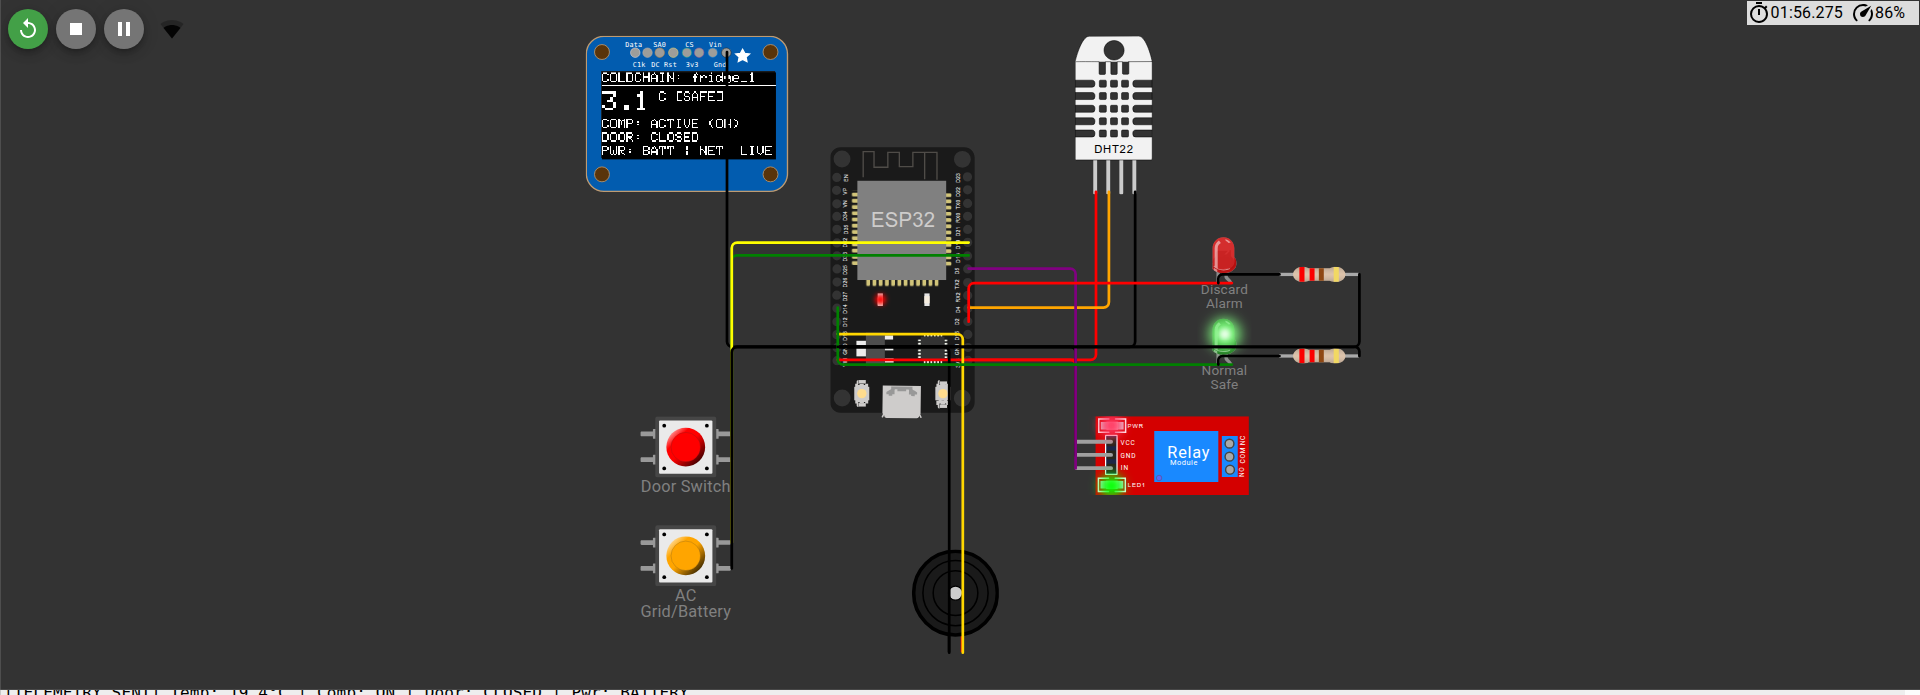
\includegraphics[width=0.92\textwidth]{images/wokwi_hardware.png}
\caption{Wokwi simulated dual-fridge node: ESP32 DevKit, DHT22 sensor, SSD1306 OLED ($3.1^\circ\text{C}$ SAFE), Compressor Relay (Active), Status LEDs, Door/Power switches, and Piezo Buzzer.}
\label{fig:wokwi_hardware}
\end{figure}

\subsection{Power Failure \& 30-Minute Edge Buffering (Task 3)}
When the power selector (GPIO 19) indicates an AC Grid blackout, the node transitions to battery backup mode, flagging \texttt{"power": "BATTERY"} in telemetry. 

During network outages (Wi-Fi or MQTT broker unreachable), the firmware shifts into offline resilience mode. Readings are pushed into a circular FIFO buffer allocated in ESP32 static RAM:
\begin{equation}
    N_{\text{capacity}} = \frac{30\,\text{min} \times 60\,\text{s/min}}{5\,\text{s/packet}} = 360\,\text{packets}
\end{equation}
Each entry encapsulates a 64-bit millisecond epoch timestamp, temperature, compressor state, door status, power source, and sequential nonce. Upon reconnecting to the MQTT broker, the firmware flushes the queued records in strictly chronological order. The server tracks received nonces to guarantee zero data loss and eliminate duplicates.

\begin{figure}[h!]
\centering
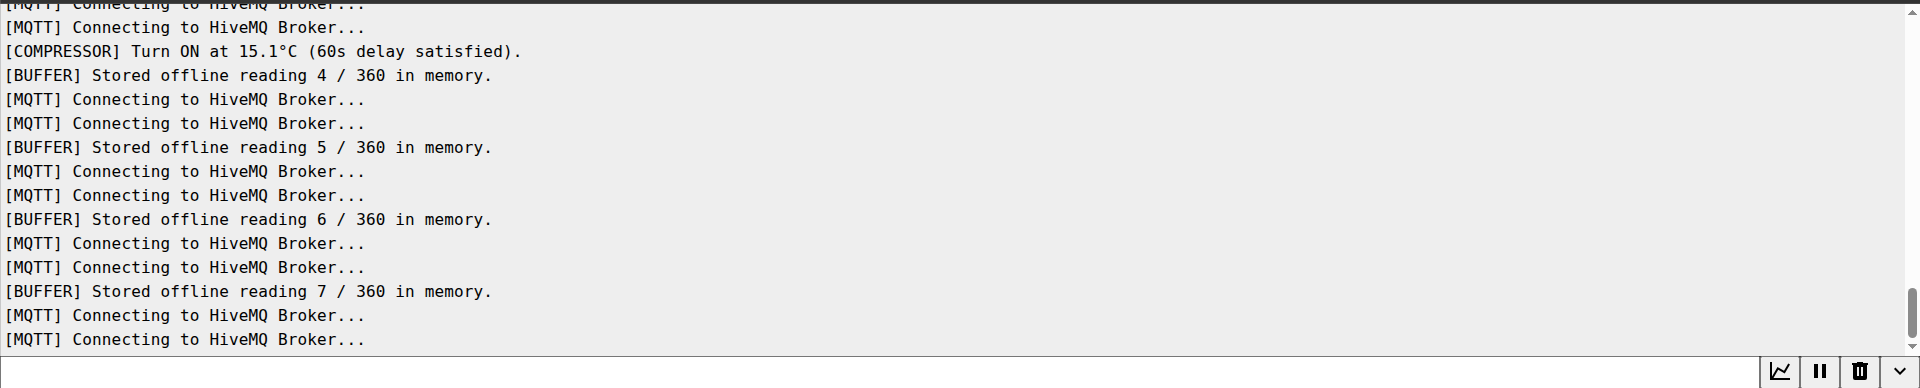
\includegraphics[width=0.92\textwidth]{images/wokwi_serial_buffer.png}
\caption{Wokwi Serial Monitor: Autonomous compressor hysteresis activation at $15.1^\circ\text{C}$ satisfying the 60s motor lockout delay, followed by offline buffer storage during network blackout.}
\label{fig:wokwi_buffer}
\end{figure}

% --- SECTION 4: HEAT-EXPOSURE BUDGET (TASK 2) ---
\section{Heat-Exposure Budget Engine (Task 2)}

Biologics deteriorate non-linearly under thermal stress. The system implements a dynamic cumulative heat-exposure budget initialized to 60.0 minutes ($3600\,\text{s}$) for each vaccine batch. 

\subsection{Degradation Kinetics \& Penalties}
When storage temperature exceeds the $8.0^\circ\text{C}$ critical threshold, the remaining budget decreases. In compliance with Arrhenius-accelerated chemical degradation kinetics, excursions exceeding $12.0^\circ\text{C}$ are penalized at double rate ($2\times$):
\begin{equation}
    \frac{dB}{dt} = \begin{cases}
        0, & T \le 8.0^\circ\text{C} \\
        -1.0, & 8.0^\circ\text{C} < T \le 12.0^\circ\text{C} \\
        -2.0, & T > 12.0^\circ\text{C}
    \end{cases}
\end{equation}

\subsection{State Transition \& Hardware Alarm Latching}
The lifecycle of every vaccine batch is evaluated continuously against three thresholds:
\begin{itemize}[leftmargin=*]
    \item \textbf{SAFE:} $B(t) > 12.0\,\text{minutes}$ ($> 20\%$). Potency certified.
    \item \textbf{AT RISK:} $0.0 < B(t) \le 12.0\,\text{minutes}$ ($\le 20\%$). Warning surfaced on dashboard; candidate for immediate relocation.
    \item \textbf{DISCARD:} $B(t) = 0.0\,\text{minutes}$ ($0\%$). Biological potency irreparably compromised.
\end{itemize}
When any batch enters the \texttt{DISCARD} state, the backend commands the ESP32 to illuminate the physical Red LED (GPIO 2). The LED remains latched in the active alarm state even if the temperature returns to the safe $2$--$8^\circ\text{C}$ range. Deactivation requires an explicit cryptographic reset command issued by an authenticated system Administrator.

\begin{figure}[h!]
\centering
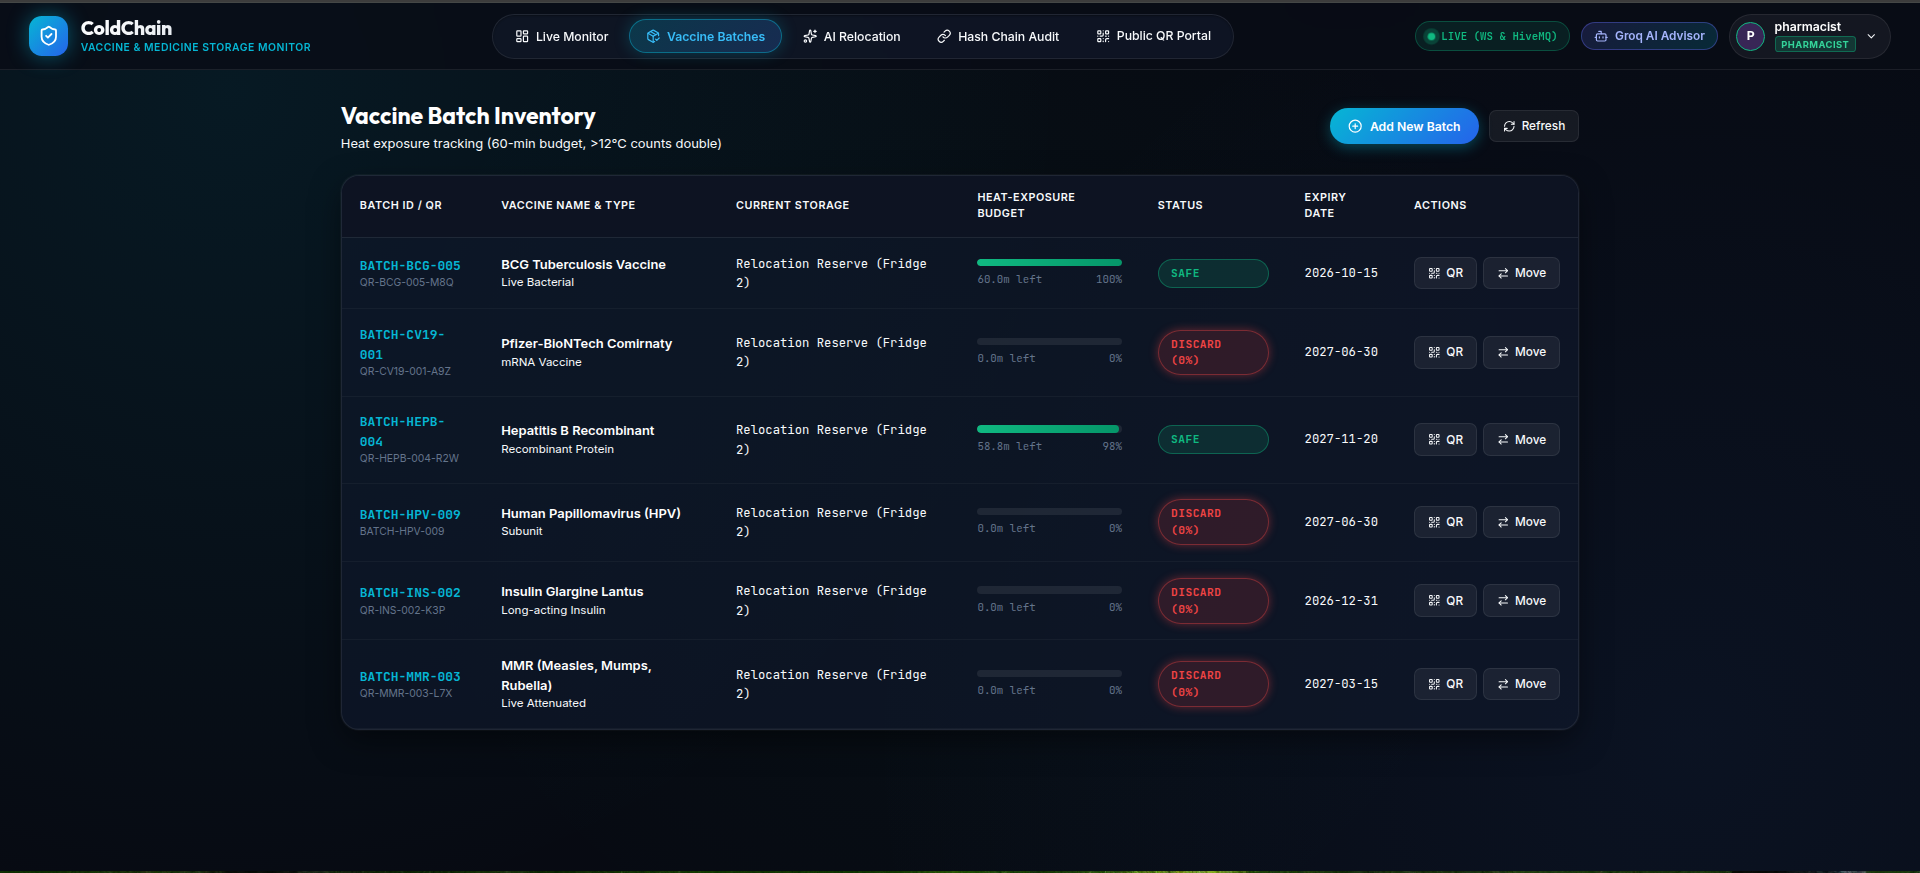
\includegraphics[width=0.92\textwidth]{images/dashboard_inventory.png}
\caption{Vaccine Batch Inventory dashboard showing real-time heat-exposure budget bars, expiry dates, clinical status (SAFE vs DISCARD), batch creation modal, and instant QR verification triggers.}
\label{fig:inventory}
\end{figure}

% --- SECTION 5: SECURITY, AUDIT & WEB APP (TASK 4) ---
\section{Web Application, Security \& Tamper-Evident Ledger (Task 4)}

\subsection{Full-Stack Architecture \& Access Control}
The web application is built on an asynchronous Node.js Express backend coupled with a responsive, single-page application frontend styled with CSS custom properties and HSL tokens. Bi-directional WebSockets (\texttt{ws://}) stream live telemetry updates to connected clients with sub-100ms latency.

Role-Based Access Control (RBAC) enforces strict authorization at the API route boundary:
\begin{itemize}[leftmargin=*]
    \item \textbf{Administrator:} Full system administration, batch creation, user provisioning, and physical hardware alarm reset.
    \item \textbf{Pharmacist:} Clinical inventory management, manual fridge-to-fridge batch transfers, and 1-click execution of AI relocation plans.
    \item \textbf{Inspector:} Read-only audit ledger inspection, cryptographic integrity verification, and compliance validation.
\end{itemize}

\subsection{Edge Security: HMAC-SHA256 \& Replay Defense}
Every telemetry packet transmitted by the ESP32 includes a message authentication code computed over a pre-shared secret key ($K$):
\begin{equation}
    \sigma = \text{HMAC-SHA256}(K, \; T \parallel \text{door} \parallel \text{pwr} \parallel \text{comp} \parallel \tau \parallel \text{nonce})
\end{equation}
Upon ingestion, the server verifies:
\begin{enumerate}[leftmargin=*]
    \item \textbf{Authenticity:} Recalculates $\sigma$ and rejects mismatched payloads with HTTP 401.
    \item \textbf{Freshness:} Rejects packets where $|\tau_{\text{server}} - \tau| > 300\,\text{seconds}$.
    \item \textbf{Uniqueness:} Maintains an in-memory sliding window of nonces; replayed tokens are discarded immediately.
\end{enumerate}

\subsection{Cryptographic Hash-Chain Audit Ledger}
To meet regulatory data integrity standards (FDA 21 CFR Part 11 and WHO Annex 9), all critical state changes (breaches, relocations, logins, resets) are appended to a linear cryptographic hash chain:
\begin{equation}
    \mathcal{H}_i = \text{SHA256}\left(i \;\|\; \tau_i \;\|\; \text{EventType}_i \;\|\; \text{Actor}_i \;\|\; \text{Payload}_i \;\|\; \mathcal{H}_{i-1}\right)
\end{equation}
The dashboard includes an interactive "Simulate DB Tamper" utility for judges and inspectors, which modifies an arbitrary database row. Clicking "Verify Integrity" causes the verification engine to traverse the chain, instantly flagging the exact block where the hash recalculation fails.

\begin{figure}[h!]
\centering
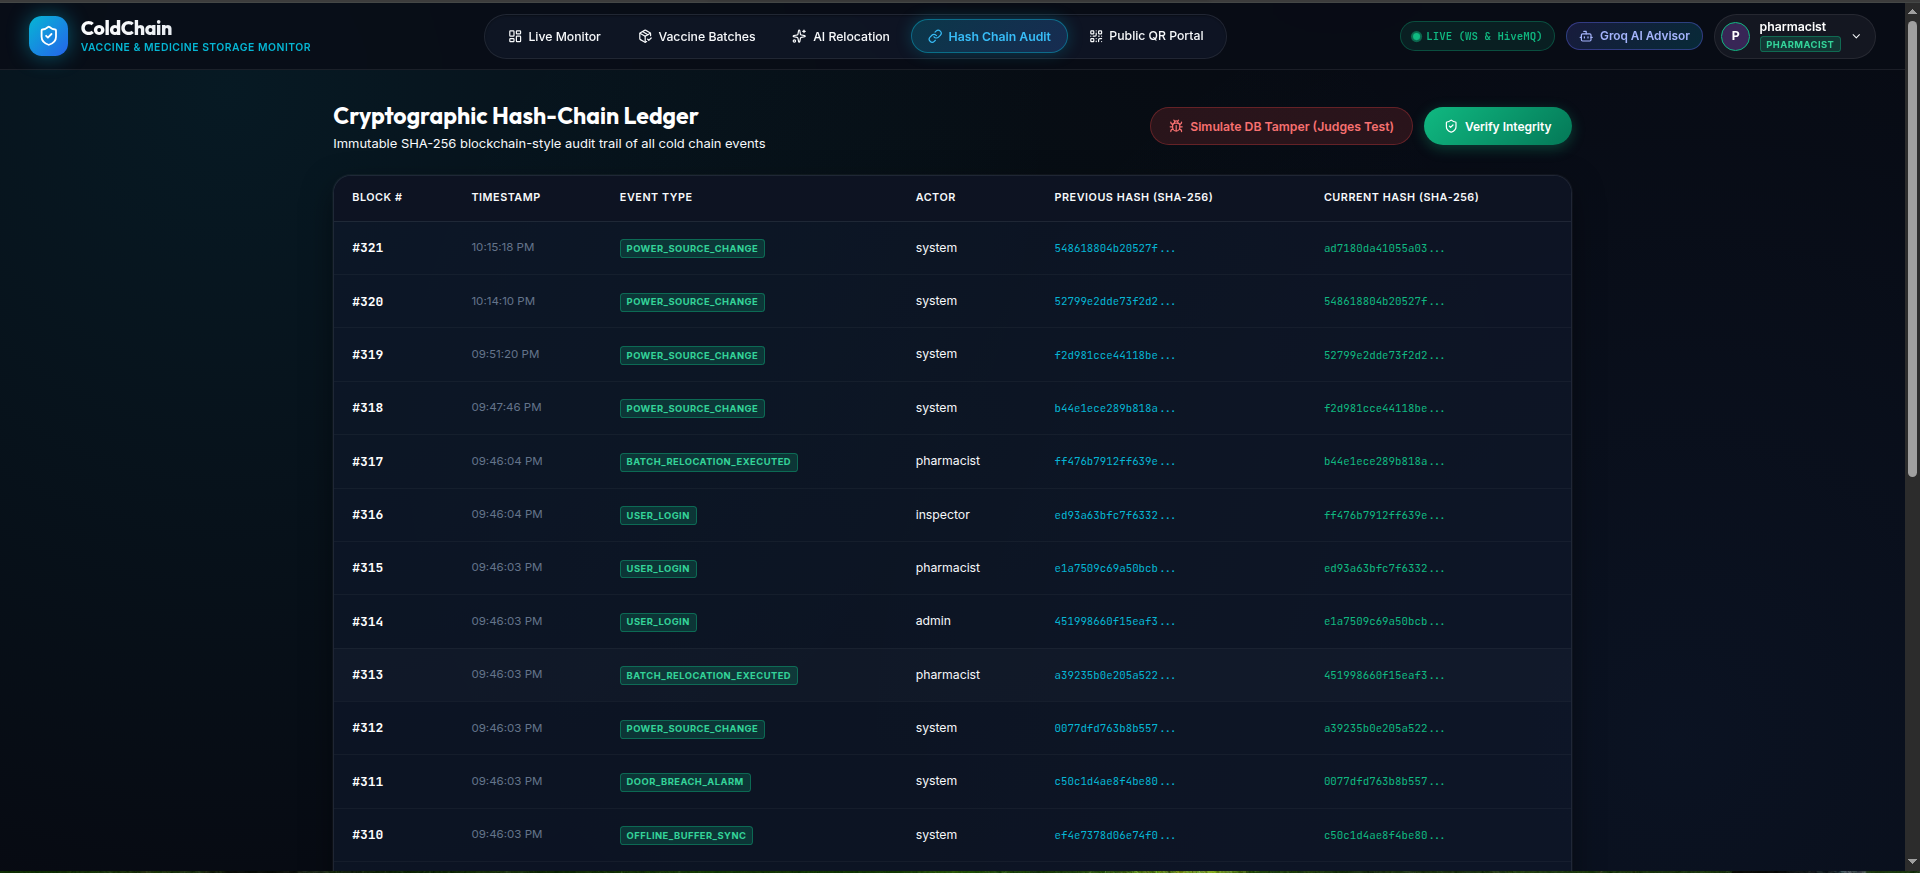
\includegraphics[width=0.92\textwidth]{images/dashboard_hashchain.png}
\caption{Cryptographic Hash-Chain Ledger: Immutable event history displaying block index, timestamp, event type, actor, previous hash, current SHA-256 hash, and the integrity verification tools.}
\label{fig:hashchain}
\end{figure}

\subsection{Public Zero-Login QR Safety Portal}
Every batch is provisioned with a standardized QR code encoding a secure public verification URL: \texttt{/verify/:batchId}. 

Field health workers, distribution couriers, or end-recipients can scan the physical vial using any smartphone camera without logging in. The responsive public portal displays the official vaccine name, manufacturer, expiration date, remaining heat budget, current storage location, and on-chain cryptographic verification status.

\begin{figure}[h!]
\centering
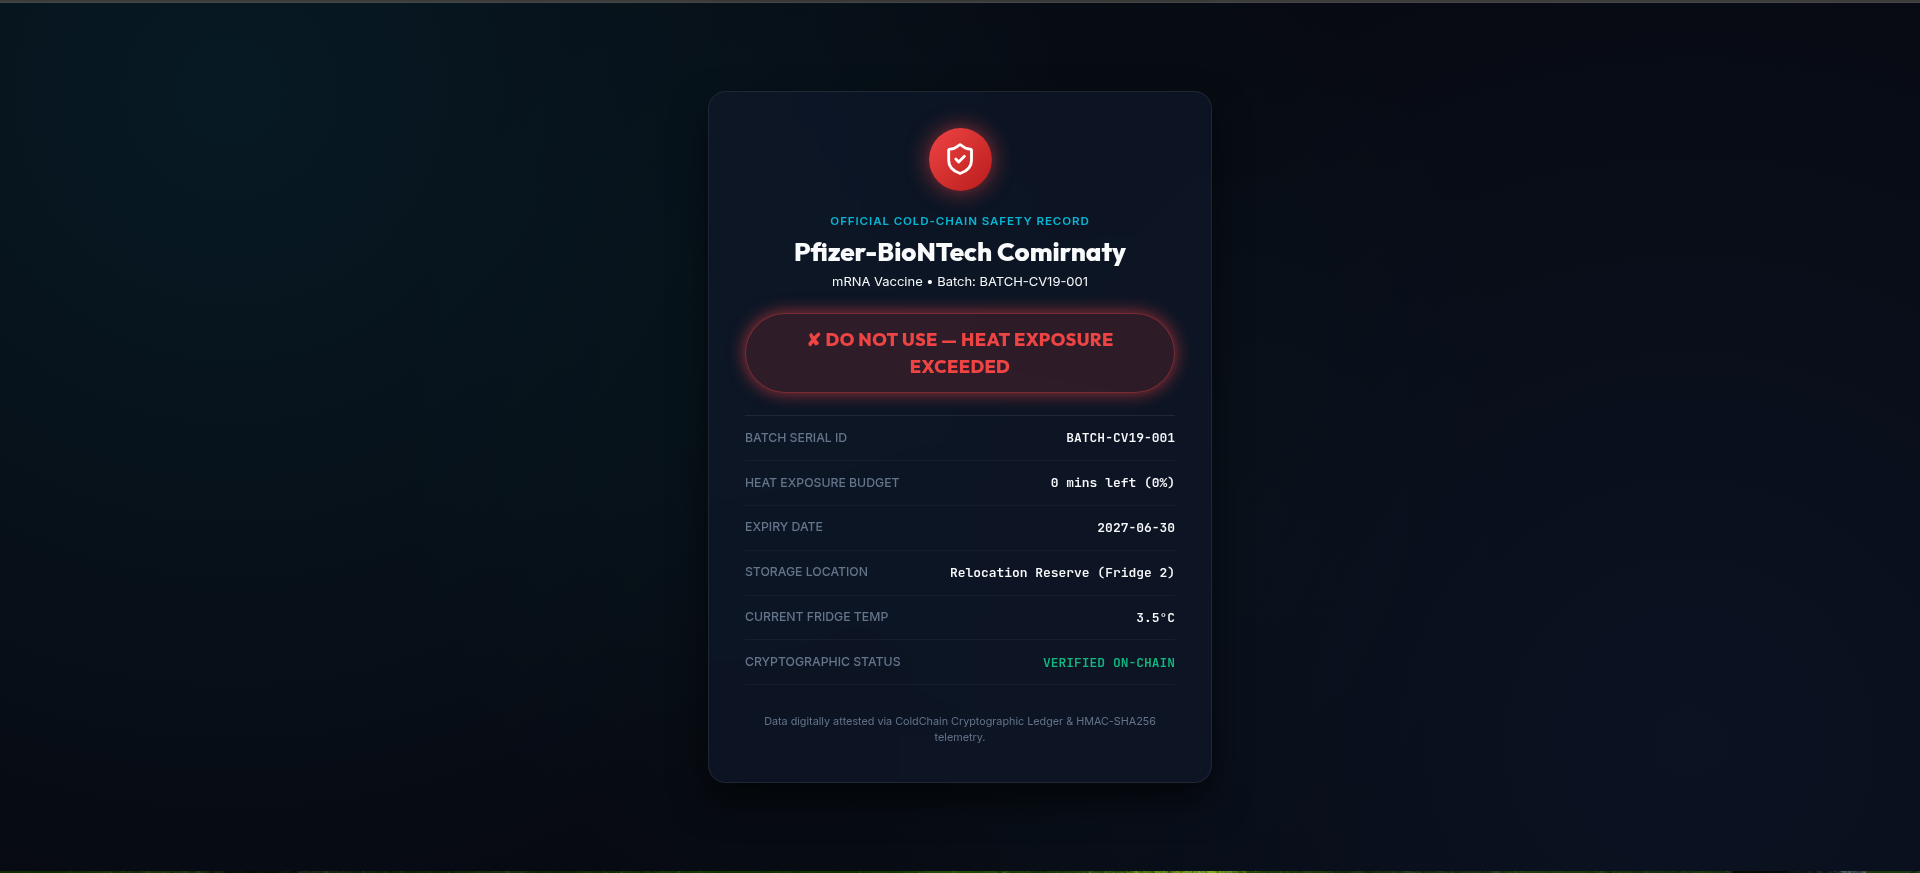
\includegraphics[width=0.65\textwidth]{images/dashboard_qr_portal.png}
\caption{Zero-Login Public QR Safety Portal showing the verified safety certificate for Pfizer-BioNTech Comirnaty (Batch BATCH-CV19-001) with explicit heat exposure exceeded warning.}
\label{fig:qr_portal}
\end{figure}

% --- SECTION 6: AI BREACH PREDICTION & RELOCATION (TASK 5) ---
\section{AI Predictive Breach \& Autonomous Relocation (Task 5)}

\subsection{30-Minute Temperature Trajectory Forecasting}
Rather than relying purely on reactive alarms, the AI engine projects temperature trajectories 30 minutes into the future. A least-squares second-order polynomial estimator fits the sliding telemetry window $[T_{t-k}, \dots, T_t]$:
\begin{equation}
    \hat{T}(t + \Delta t) = \alpha \Delta t^2 + \beta \Delta t + T(t), \quad \text{where } \Delta t = 30\,\text{min}
\end{equation}
If the extrapolated temperature $\hat{T}(t + 30\,\text{min}) > 8.0^\circ\text{C}$, the system issues an early warning on the live dashboard well before the physical breach occurs, providing staff an operational window for preventative intervention.

\begin{figure}[h!]
\centering
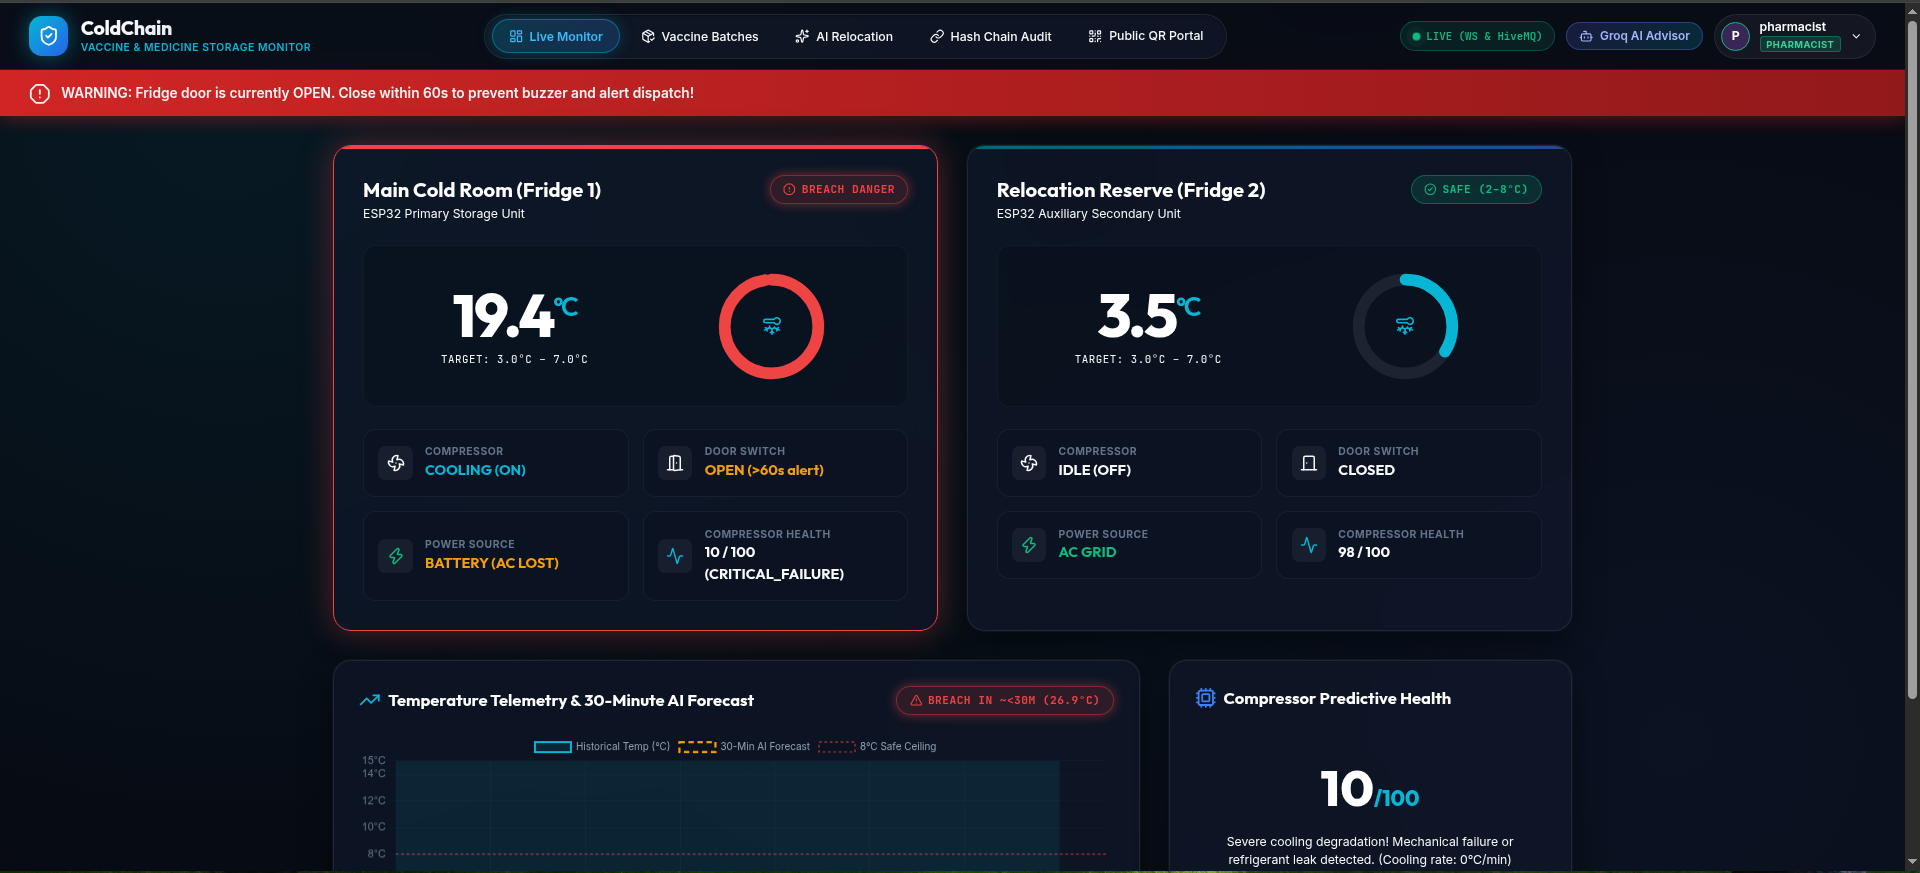
\includegraphics[width=0.92\textwidth]{images/dashboard_live_breach.png}
\caption{Live Monitor Dashboard during simulated emergency: Fridge 1 at $19.4^\circ\text{C}$ under battery backup with door open alert, 30-min AI prediction warning ($26.9^\circ\text{C}$), and degraded compressor health ($10/100$).}
\label{fig:live_breach}
\end{figure}

\subsection{Compressor Health Degradation Scoring (0--100)}
The health score evaluates thermodynamic cooling performance when the compressor relay is energized. The observed rate of cooling is computed as:
\begin{equation}
    R_{\text{cool}} = \left| \frac{\Delta T}{\Delta t} \right|_{\text{Compressor}=\text{ON}}
\end{equation}
Under nominal conditions, clean refrigeration systems yield $R_{\text{cool}} \ge 0.5^\circ\text{C}/\text{min}$, corresponding to a Health Score of $100/100$. When refrigerant leaks, coil fouling, or motor wear degrade performance ($R_{\text{cool}} \le 0.1^\circ\text{C}/\text{min}$), the health score drops below $20/100$, triggering a \texttt{CRITICAL\_FAILURE} status.

\subsection{Autonomous Relocation Algorithm \& 1-Click Confirmation}
When a primary fridge exhibits a predicted thermal breach or critical compressor degradation, the relocation engine evaluates candidate secondary units (Fridge 2). The algorithm verifies:
\begin{enumerate}[leftmargin=*]
    \item Target unit current temperature $T_{\text{target}} \le 5.0^\circ\text{C}$.
    \item Target compressor health score $\ge 80/100$.
    \item Storage slot availability for the at-risk batches.
\end{enumerate}
The generated relocation plan is displayed on the pharmacist's console. With a single click on "Execute Relocation Protocol", the batch records are transferred atomically in the database, logged to the hash chain, and updated across the live digital twins.

\begin{figure}[h!]
\centering
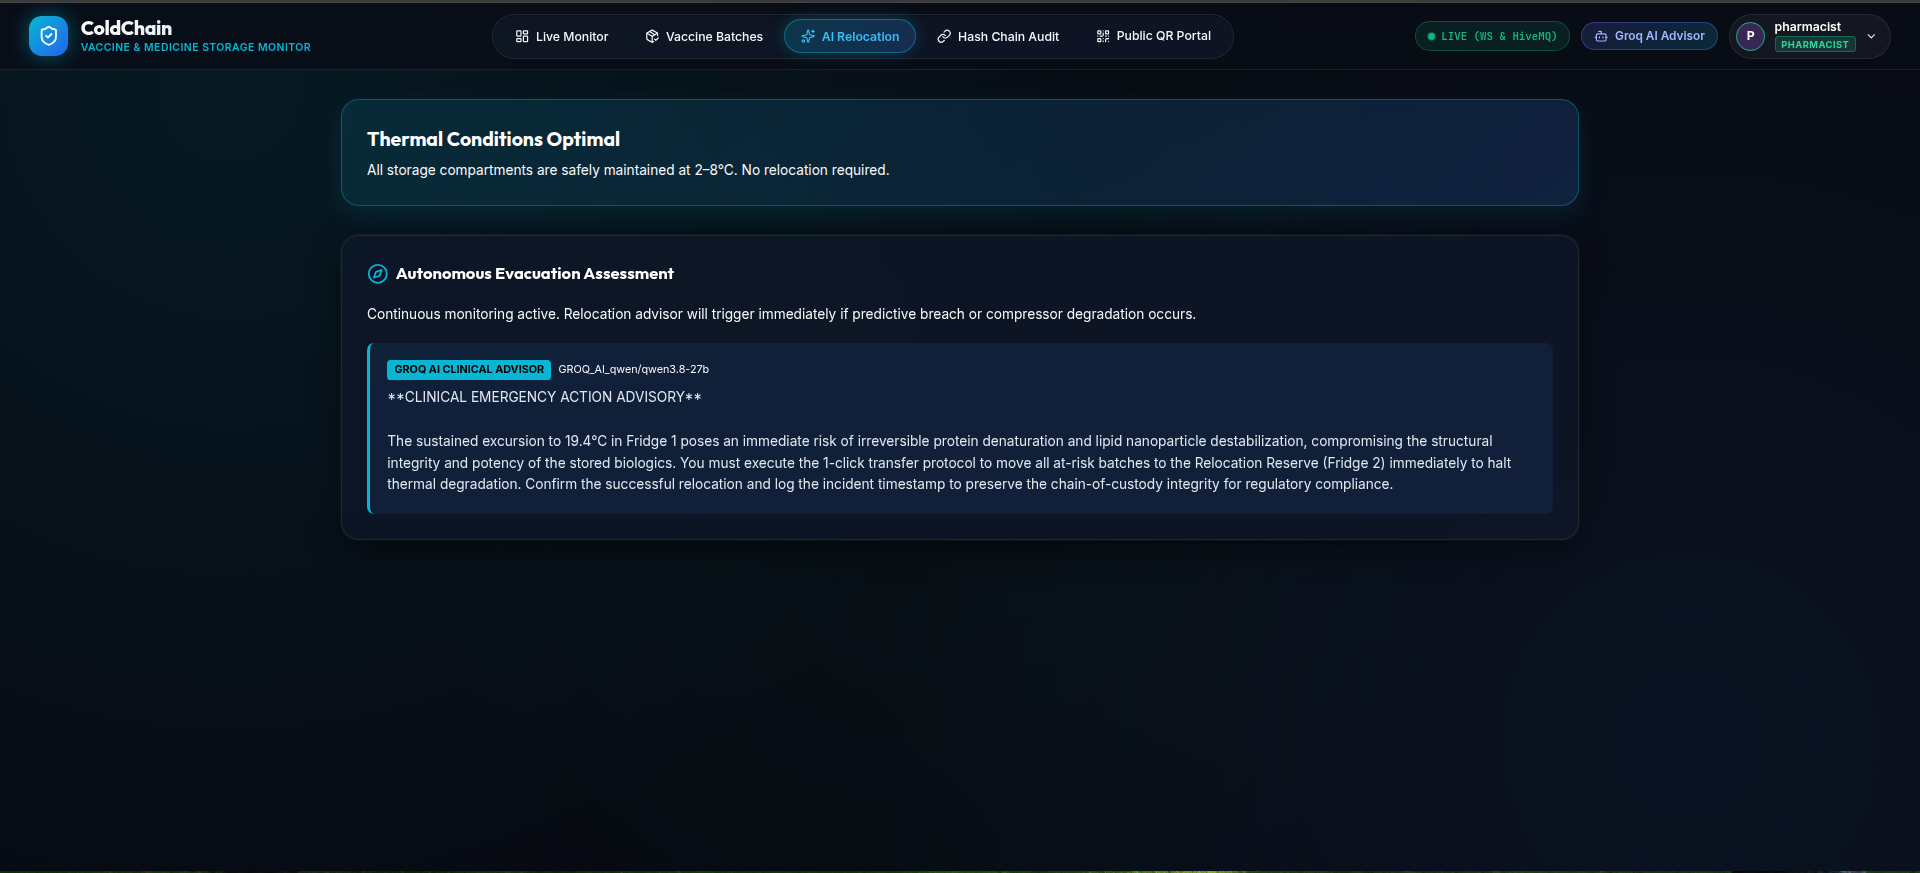
\includegraphics[width=0.92\textwidth]{images/dashboard_ai_relocation.png}
\caption{AI Relocation console featuring the Autonomous Evacuation Assessment and real-time clinical guidance generated by the integrated Groq Cloud LLM (Qwen 3.8-27B).}
\label{fig:ai_relocation}
\end{figure}

\subsection{Groq Cloud LLM Clinical Emergency Advisor}
An integration with Groq Cloud accelerates inference using the Qwen 3.8-27B model. During thermal excursion events, the advisor analyzes the exact temperature history, elapsed excursion time, and biologics profile (mRNA vs live-attenuated vs recombinant) to generate clinical directives covering protein denaturation risks and handling procedures.

% --- SECTION 7: EXPERIMENTAL VERIFICATION & TEST RESULTS ---
\section{Experimental Verification \& Test Results}

The complete system underwent rigorous automated test verification using Mocha and Chai assertion suites. The suite covers all five competition tasks across 33 automated test cases, executing in under 3.2 seconds.

\begin{table}[h!]
\centering
\small
\renewcommand{\arraystretch}{1.2}
\begin{tabularx}{\textwidth}{l l p{8.5cm} c}
\toprule
\textbf{Task Suite} & \textbf{Tests} & \textbf{Core Invariants Verified} & \textbf{Result} \\
\midrule
Phase 1 & 11 / 11 & JWT creation, bcrypt verification, RBAC permissions, Fridge state persistence, Batch initialization, Telemetry schema validity. & \textbf{PASSED} \\
\addlinespace
Phase 2 & 10 / 10 & 60-min heat budget decay, $2\times$ rate $>12^\circ\text{C}$, At Risk/Discard transitions, offline buffer FIFO ordering, deduplication, door $>60\text{s}$ alert, power failure detection. & \textbf{PASSED} \\
\addlinespace
Phase 3 & 7 / 7 & HMAC-SHA256 validation, timestamp freshness window, replay attack rejection, SHA-256 hash-chain creation, and deliberate tampering detection. & \textbf{PASSED} \\
\addlinespace
Phase 4 & 5 / 5 & 30-min AI polynomial extrapolation ($>8^\circ\text{C}$ alert), compressor cooling rate calculation (0--100), relocation recommendations, 1-click execution. & \textbf{PASSED} \\
\midrule
\textbf{Total} & \textbf{33 / 33} & \textbf{End-to-End System Integration Verified Across All 5 Challenge Tasks} & \textbf{100\%} \\
\bottomrule
\end{tabularx}
\caption{Summary of automated integration test suite results.}
\label{tab:test_results}
\end{table}

% --- SECTION 8: CONCLUSION & SUBMISSION CHECKLIST ---
\section{Conclusion \& Submission Package}

The ColdChain solution by \textbf{Team UFTB-VORQEN} provides a complete, robust, and mathematically sound answer to the BUBT FastRobox 1.0 IoT Hackathon Challenge. By combining embedded edge autonomy (ESP32 hysteresis and 30-minute offline buffering), cryptographic security (HMAC-SHA256 and immutable audit hash chains), predictive AI modeling (temperature forecasting and compressor diagnostics), and an accessible public inspection interface, the system ensures end-to-end biological viability across the entire medical distribution cold chain.

\subsection{Submission Artifacts \& Links}
\begin{itemize}[leftmargin=*]
    \item \textbf{GitHub Repository:} \url{https://github.com/Masud744/FastRobox1.0_Hackathon}
    \item \textbf{Wokwi Live Simulation:} \url{https://wokwi.com/projects/430889982464003073}
    \item \textbf{Local Web Application:} \texttt{http://localhost:5000} (Credentials: \texttt{admin} / \texttt{admin123}, \texttt{pharmacist} / \texttt{pharma123}, \texttt{inspector} / \texttt{inspect123})
    \item \textbf{Cloud Database:} Supabase PostgreSQL 17 mirrored instance.
\end{itemize}

\end{document}
